\documentclass[final]{jaes}

\usepackage{amsmath}
\usepackage{bm}
\DeclareMathOperator*{\argmax}{arg\,max}

% Pull generated table rows in with the primitive \input, which is expandable;
% LaTeX's \input would end the alignment row and break a following \midrule.
\makeatletter
\newcommand{\inputrows}[1]{\csname @@input\endcsname #1 }
\makeatother
\usepackage{microtype}
\usepackage{booktabs}
\usepackage{url}
\hypersetup{
  pdftitle={Measurement Context as Part of the Result: A Calibration-Aware, Reproducible Workflow for Long-Duration Acoustic Analysis},
  pdfauthor={Colby Leider},
  pdfsubject={JAES engineering-report draft},
  pdfkeywords={acoustic measurement, audio analysis, calibration, reproducibility, soundscape}
}

% Every quantity quoted in this paper is defined in results/numbers.tex, which
% is written by paper/evaluation.py.  No value below is transcribed by hand.
% Generated by paper/evaluation.py -- do not edit by hand.
\newcommand{\eslCommit}{1a34208dc2fe}
\newcommand{\eslCommitFull}{1a34208dc2fe8a619110fdb4db806202a6ca83b8}
\newcommand{\eslSeed}{20260906}
\newcommand{\eslPython}{3.11.15}
\newcommand{\eslNumpy}{2.4.6}
\newcommand{\eslSoundfile}{0.14.0}
\newcommand{\eslPlatform}{Linux-6.18.44-fc-v24-x86\_64-with-glibc2.39}
\newcommand{\eslMetricTotal}{75}
\newcommand{\eslMetricStreaming}{37}
\newcommand{\dispCombos}{84}
\newcommand{\dispRange}{15.9}
\newcommand{\dispMin}{84.2}
\newcommand{\dispMax}{100.1}
\newcommand{\dispStd}{4.1}
\newcommand{\dispConservativeCombos}{48}
\newcommand{\dispConservativeRange}{8.1}
\newcommand{\dispTopAxis}{Time aggregation}
\newcommand{\dispTopAxisRange}{11.8}
\newcommand{\anaCases}{24}
\newcommand{\anaFrame}{2048}
\newcommand{\anaRmsErr}{$3.3\times10^{-4}$}
\newcommand{\anaPeakErr}{$1.4\times10^{-5}$}
\newcommand{\anaCrestErr}{$3.3\times10^{-4}$}
\newcommand{\anaCentroidOn}{0.0174}
\newcommand{\anaCentroidOff}{0.546}
\newcommand{\anaCentroidRatio}{31}
\newcommand{\decayCases}{24}
\newcommand{\decayCleanErr}{$8.7\times10^{-7}$}
\newcommand{\decayWorstPct}{1583}
\newcommand{\decayDegraded}{9}
\newcommand{\decayDegradedFlagged}{9}
\newcommand{\valCases}{36}
\newcommand{\valExpected}{18}
\newcommand{\valCorrect}{18}
\newcommand{\valMissed}{0}
\newcommand{\valFalseAlarms}{0}
\newcommand{\valCorrectReported}{18}
\newcommand{\streamChecked}{18}
\newcommand{\streamIdentical}{yes}
\newcommand{\streamLegacyMissing}{8.2}
\newcommand{\streamLegacyMissingMin}{0.7}
\newcommand{\streamLegacyWorstRel}{2.33}
\newcommand{\memBaseline}{384}
\newcommand{\memFloor}{384}
\newcommand{\memFloorBelow}{60}
\newcommand{\memFitPoints}{9}
\newcommand{\memPredictedSubset}{2.93}
\newcommand{\memFullSlope}{3.31}
\newcommand{\memFullIntercept}{118}
\newcommand{\memFullRsq}{1.0000}
\newcommand{\memStreamSlope}{0.000}
\newcommand{\memStreamIntercept}{384}
\newcommand{\memPredicted}{4.40}
\newcommand{\memDataRateMultiple}{9}
\newcommand{\memFullHour}{11.7}
\newcommand{\memStreamHour}{0.38}
\newcommand{\memFullDay}{279}
\newcommand{\memMaxDuration}{480}
\newcommand{\memDurations}{15, 30, 60, 120, 240, 480}
\newcommand{\calFixtures}{6}
\newcommand{\calTolerance}{0.001}
\newcommand{\calAchieved}{$2.5\times10^{-7}$}
\newcommand{\evtCleanMedian}{8.2}
\newcommand{\evtCleanPninetyfive}{13.7}
\newcommand{\evtNoisyMedian}{5.3}
\newcommand{\evtNoisyPninetyfive}{3.0}
\newcommand{\evtNoiseRateStep}{40}
\newcommand{\evtNoiseMedianStep}{0.9}
\newcommand{\evtCleanMedianStep}{4.3}
\newcommand{\evtCleanMedianNoise}{4.2}
\newcommand{\evtCleanRate}{100}
\newcommand{\evtNoisyRate}{78}
\newcommand{\evtHopMs}{16}
\newcommand{\evtTrials}{40}


\sptitle{REPRODUCIBLE LONG-DURATION ACOUSTIC ANALYSIS}
\title{Measurement Context as Part of the Result: A Calibration-Aware, Reproducible Workflow for Long-Duration Acoustic Analysis}

\authorgroup{
  \author{COLBY LEIDER}
  \email{colbyleider@gmail.com}
  \affil{ecoSignalLab Project, United States}
}

\abstract{A sound level reported without its weighting, time aggregation, framing, channel policy, and calibration path is not a measurement but a number. This report quantifies what that omission costs and describes ecoSignalLab, an open-source Python workflow that binds each value to the choices that produced it. Analysing one 30-second scene under \dispCombos{} individually defensible but undocumented combinations of those choices produced reported levels spanning \dispRange~dB; holding the time statistic fixed so that only nominally immaterial choices vary still leaves \dispConservativeRange~dB, of which frequency weighting alone contributes \dispTopAxisRange~dB. The workflow applies a common result contract to \eslMetricTotal{} metrics, of which \eslMetricStreaming{} support chunked execution. A self-audit conducted for this paper found that the metric previously published as interchannel coherence was a zero-lag correlation returning negative values; it has been renamed and a magnitude-squared coherence added, and the two now correctly disagree on a delayed channel pair. Against a suite of degenerate inputs the validity fields reported a measurement as unavailable in \valCorrect{} of \valExpected{} cases that warranted it, with \valFalseAlarms{} false alarms. Introducing a frame-aligned streaming path with boundary continuity made chunked analysis bit-identical to full-file analysis for all \streamChecked{} metric-by-chunk-size comparisons, where independent chunking had discarded up to \streamLegacyMissing\% of frames. Peak memory for full-file analysis grows at \memFullSlope~MiB per second of stereo audio, about \memDataRateMultiple{} times the raw data rate, implying roughly \memFullHour~GiB for one hour, while the streaming path stays at \memStreamIntercept~MiB. The evaluation script, intermediate tables, and figures are provided for reproduction.}

\begin{document}

\maketitle

\begin{keywords}
Acoustic measurement, audio analysis, calibration, reproducibility, soundscape
\end{keywords}

\section{INTRODUCTION}

Acoustic monitoring has moved from short, purpose-built measurements toward persistent recordings made by autonomous, networked, and multichannel systems. Such recordings are used to describe habitats, rooms, products, and listening environments. They also create an engineering problem: the signal may be large, the channel layout may be ambiguous, and the interpretation of a reported level depends on calibration information that is often stored separately from the audio. Earlier multisensor field systems already exposed the need to join sensor state and acoustic evidence \cite{leider2010}. Contemporary soundscape research extends that need across much larger collections \cite{krause2008,pijanowski2011,merchant2015}.

The required signal-processing components are familiar. Short-time Fourier analysis supports spectral descriptors \cite{allen1977}; correlation-based estimators support delay measurement \cite{knapp1976,carter1987}; integrated decay curves support reverberation-time estimation \cite{schroeder1965}; and spectral-flux functions can expose structural transitions \cite{dixon2006,bello2005}. The engineering difficulty lies in composing these components without silently changing channel meaning, units, framing, or calibration assumptions. A single scalar in a comma-separated file is not self-interpreting: ``$72$~dB'' is incomplete unless the reference, weighting, time integration, calibration path, and aggregation are known.

That claim is usually asserted and rarely priced. Section~\ref{sec:dispersion} prices it. Analysing one recording under every combination of a small set of choices that a competent engineer might make without documenting them --- frame length, frequency weighting, time aggregation, channel policy --- produced reported levels spanning \dispRange~dB. Even with the time statistic held fixed, so that no one can object that $L_{\mathrm{max}}$ and $L_{90}$ are simply different quantities, the spread is \dispConservativeRange~dB. A number of that size is the difference between compliance and violation in most noise ordinances, and it is invisible in any report that gives the level alone.

Existing soundscape studies also caution against treating broad acoustic indices as direct labels for sources or ecological outcomes \cite{sueur2014,bradfer2019}. Perceptual soundscape segmentation further shows that foreground/background organization matters in addition to aggregate spectra \cite{thorogood2016}. In privacy-sensitive monitoring, retained features may be preferable to retained speech-bearing audio, but only if their generation remains auditable \cite{bitzer2016}. ISO 12913-2 makes the point normative for soundscape work by specifying what must be reported alongside a measurement \cite{iso12913-2}. These concerns motivate a workflow in which measurement context is part of the result rather than an informal note.

This paper describes and verifies the implementation of ecoSignalLab, a Python package intended to make heterogeneous acoustic analysis inspectable and rerunnable. Its engineering contributions are: (1) a registry of \eslMetricTotal{} metrics behind a shared contract; (2) explicit, testable policies for frames, channels, calibration, and validity; (3) a bounded-memory streaming path that is numerically identical to full-file analysis for its \eslMetricStreaming{} stream-compatible metrics; and (4) a provenance record that binds outputs to configuration and software state. Each of the four is evaluated rather than merely described, and Sec.~\ref{sec:limits} states plainly where the evaluation stops.

\section{ENGINEERING REQUIREMENTS}

\subsection{Measurement Context and Traceability}

Reproducible computational work requires the data, transformations, and parameters needed to regenerate a result \cite{sandve2013}. The FAIR principles additionally emphasize findability, accessibility, interoperability, and reuse \cite{wilkinson2016}. For acoustic measurements, a useful minimum record includes the decoder and sample format, sample rate, channel count and labels, frame and hop sizes, window, selected metrics, calibration mode, weighting, deterministic seed, package versions, and warnings.

For soundscape work this minimum is not a matter of taste. ISO 12913-2 specifies the data and metadata to be reported with a soundscape measurement, and ISO 12913-3 addresses subsequent analysis \cite{iso12913-2,iso12913-3}. Table~\ref{tab:iso} maps the machine-readable portion of that requirement onto the provenance record described in Sec.~\ref{sec:provenance}. The rows the software cannot fill are as informative as the rows it can: source, receiver geometry, and observer context are operator knowledge, and a workflow that silently omitted them would be claiming a completeness it does not have.

Traceability is especially important for sound level. A digital full-scale measurement can be reported directly in dBFS. A physical sound-pressure level requires a mapping from samples to pascals, either through a reference recording or through an instrumentation chain. A-weighted, C-weighted, and Z-weighted results must remain distinguishable, and an analysis tool should not imply IEC meter compliance merely because it implements a corresponding frequency response \cite{iec61672}. Likewise, programme loudness according to Recommendation ITU-R BS.1770 is a defined procedure rather than a synonym for average digital level \cite{itu1770}.

\begin{table}[t]
\caption{ISO 12913-2 REPORTING ITEMS AGAINST THE PROVENANCE RECORD}
\label{tab:iso}
\centering
\small
\begin{tabular}{@{}p{0.44\columnwidth}p{0.48\columnwidth}@{}}
\toprule
Reporting item & Provenance field \\
\midrule
Recording format, sample rate, bit depth & \texttt{decoder}, \texttt{subtype}, \texttt{sample\_rate} \\
Channel count and layout & \texttt{channel\_summary}, \texttt{spatial\_metadata} \\
Calibration method and reference & \texttt{calibration} (path, $K$, chain) \\
Frequency weighting & propagated into metric name and units \\
Time weighting / integration & \texttt{frame\_size}, \texttt{hop\_size}, metric identity \\
Analysis software and version & \texttt{esl\_version}, \texttt{library\_versions}, \texttt{pipeline\_hash} \\
Measurement uncertainty & \emph{not captured}; requires chain characterization \\
Source and receiver geometry & \emph{not captured}; operator entry \\
Site description, observer context & \emph{not captured}; operator entry \\
\bottomrule
\end{tabular}
\end{table}

\subsection{Related Tools}

The components above exist in several mature packages, so the question a reader should ask is what this workflow adds. Table~\ref{tab:related} answers it directly. Broad feature coverage is common; what is uncommon is emitting, with every value, a machine-readable record of the calibration state, channel resolution, framing, and validity that produced it, such that a downstream consumer can tell a measured zero from an unavailable measurement without consulting the operator.

\begin{table*}[t]
\caption{RELATED OPEN-SOURCE ACOUSTIC ANALYSIS PACKAGES. CAL.: PHYSICAL-LEVEL CALIBRATION. VAL.: PER-VALUE VALIDITY FIELDS. PROV.: MACHINE-READABLE PROVENANCE RECORD. STR.: BOUNDED-MEMORY STREAMING.}
\label{tab:related}
\centering
\small
\begin{tabular}{@{}llcccll@{}}
\toprule
Package & Language & Cal. & Val. & Prov. & Str. & Primary focus \\
\midrule
librosa \cite{mcfee2015} & Python & no & no & no & no & music and audio feature extraction \\
scikit-maad \cite{ulloa2021} & Python & partial & no & no & no & ecoacoustic indices \\
seewave / soundecology \cite{sueur2008} & R & partial & no & no & no & ecoacoustic indices \\
OpenSoundscape \cite{lapp2023} & Python & no & no & partial & partial & supervised bioacoustics \\
pyloudnorm \cite{steinmetz2021} & Python & n/a & no & no & no & programme loudness (BS.1770) \\
ecoSignalLab (this work) & Python & yes & yes & yes & yes & general acoustic description \\
\bottomrule
\end{tabular}
\end{table*}

\subsection{Long-Duration and Multichannel Constraints}

For $C$ channels, $N$ samples, and $M$ simultaneous time series, memory consumption can become more restrictive than arithmetic cost. Loading an entire recording, materializing a spectrogram, and retaining every metric series gives memory that grows with duration; Sec.~\ref{sec:memory} measures that growth and accounts for it component by component. A streaming alternative should bound resident state, and --- this is the stronger requirement --- it should not change the numbers.

Channel operations introduce a second axis of ambiguity. A mono reduction, per-channel measurement, paired-channel descriptor, and first-order ambisonic operation do not represent interchangeable views of the same signal. Interchannel coherence, interaural cross-correlation coefficient (IACC), interchannel level difference (ILD), and interchannel time difference (ITD) require at least two channels and an explicit pair. Spatial metadata should therefore be resolved before a metric is scheduled, and a pair inferred from channel count must be recorded as an inference rather than a fact.

\subsection{A Common Result Contract}

The workflow was designed around four requirements. First, each metric declares prerequisites and returns value, unit, summary, series, and validity fields in a common schema. Second, failures remain local: an unsupported metric is marked invalid with a reason instead of invalidating unrelated measurements. Third, users can request only the required metrics or a named profile. Fourth, JSON and tabular exports preserve the context needed to interpret their values.

\section{SYSTEM DESIGN}

\subsection{Analysis Pipeline}

The core pipeline decodes audio to a floating-point array with shape $[N,C]$. Unless overridden, it forms $2048$-sample frames at a $512$-sample hop. A shared analysis context exposes the waveform, sample rate, channel policy, frame coordinates, and lazily computed spectral quantities. Reusing the context prevents independent plugins from decoding the same file or computing identical transforms.

For a frame $x_c[n]$ on channel $c$, the digital RMS level is
\begin{equation}
L_{\mathrm{RMS,FS},c}=20\log_{10}\left(
\sqrt{\frac{1}{N_f}\sum_{n=0}^{N_f-1}x_c^2[n]}+\epsilon_{\mathrm{lvl}}\right),
\label{eq:rms}
\end{equation}
where $N_f$ is the frame length and $\epsilon_{\mathrm{lvl}}=10^{-12}$ prevents an undefined logarithm for digital silence, imposing a level floor near $-240$~dBFS. Spectral descriptors are computed from a windowed short-time Fourier transform in which every magnitude bin carries an additive floor $\epsilon_{\mathrm{mag}}=10^{-12}$. For magnitude $X[k,m]$ at frequency $f_k$, the spectral centroid is
\begin{equation}
f_{\mathrm{c}}[m]=\frac{\sum_k f_k |X[k,m]|}{\sum_k |X[k,m]|}.
\label{eq:centroid}
\end{equation}
Both floors are recorded in the provenance document. This is not pedantry: an unstated constant inside a decibel computation is exactly the kind of hidden choice this paper argues against, and Sec.~\ref{sec:validity} shows that $\epsilon_{\mathrm{mag}}$ alone was enough to make Eq.~\eqref{eq:centroid} return a confident $12$~kHz for digital silence until the silence test described there was added.

The implementation groups \eslMetricTotal{} registered metrics into the categories shown in Table~\ref{tab:catalog}. The count is a software inventory, not a claim that all metrics are statistically independent or equally appropriate for every signal; several entries are families distinguished by weighting, channel operation, or aggregation, and the complete registry, with units, defining reference, streaming capability, and validity conditions per entry, is distributed with the repository rather than reproduced here. Of the \eslMetricTotal{}, \eslMetricStreaming{} declare compatibility with chunked execution.

\begin{table}[t]
\caption{REGISTERED METRIC CATALOG AT THE EVALUATED COMMIT}
\label{tab:catalog}
\centering
\begin{tabular}{@{}lr@{}}
\toprule
Category & Count\\
\midrule
Anomaly / novelty & 6\\
Architectural acoustics & 13\\
Basic & 11\\
Ecoacoustics & 7\\
Level and loudness & 20\\
Noise and SNR & 1\\
Spatial & 10\\
Spectral & 6\\
Temporal & 1\\
\midrule
Total & \eslMetricTotal\\
\bottomrule
\end{tabular}
\end{table}

The ecoacoustic group includes acoustic complexity, diversity, evenness, bioacoustic activity, entropy, and normalized difference soundscape measures. Such values are treated as signal summaries under named band definitions, not as direct biodiversity estimates. This distinction follows published guidance on acoustic-index interpretation \cite{pieretti2011,sueur2014,bradfer2019}.

\subsection{Calibration Model}

The first supported physical-level path is a reference offset. If a reference tone with known sound-pressure level $L_{\mathrm{ref,SPL}}$ measures $L_{\mathrm{ref,FS}}$, then
\begin{equation}
K=L_{\mathrm{ref,SPL}}-L_{\mathrm{ref,FS}}, \qquad
L_{\mathrm{SPL}}=L_{\mathrm{FS}}+K.
\label{eq:offset}
\end{equation}
The result records both levels and $K$. The second path derives a scale from microphone sensitivity, preamplifier gain, and analog-to-digital converter full-scale voltage. These parameters are stored with the result so that the physical-level claim is inspectable. If neither path is supplied, the system retains dBFS and explicitly marks SPL as unavailable.

Frequency weighting is represented by the standard analytic magnitude responses. The weighting label is propagated into metric names, units, and provenance. This implementation is suitable for repeatable signal analysis, but the software does not model a complete certified sound-level meter, calibration laboratory uncertainty, microphone free-field corrections, or instrument tolerances. Consequently, its weighted levels must not be presented as standards-certified measurements without independent validation of the complete measurement chain.

\subsection{Streaming with Frame Continuity}
\label{sec:streaming-design}

The streaming path reads fixed-size chunks and executes only metrics whose plugins declare chunk compatibility. For each scalar stream $x_i$, the mean and variance are updated with the numerically stable recurrence described by Welford \cite{welford1962}:
\begin{equation}
\begin{aligned}
\delta_i &= x_i-\mu_{i-1}, &
\mu_i &= \mu_{i-1}+\frac{\delta_i}{i},\\
M_{2,i} &= M_{2,i-1}+\delta_i(x_i-\mu_i).&&
\end{aligned}
\label{eq:welford}
\end{equation}
Minimum, maximum, and count are exact for the values presented to the accumulator. Quantiles use a deterministic reservoir of at most 8192 values, following the general reservoir-sampling principle \cite{vitter1985}. In summary-only mode, per-frame series are discarded after aggregation.

An earlier revision of this implementation analysed each chunk independently, framing it from its own sample zero. That is worse than it sounds. Frames straddling a chunk boundary are never computed, and, because a chunk length is generally not an integer multiple of the hop, the analysis grid is re-anchored at every chunk, so the streamed frame set is not even a subset of the full-file frame set. Section~\ref{sec:streaming} quantifies both effects.

The evaluated implementation instead re-blocks the stream onto the global frame grid. Chunk $k$ is emitted so that its first frame begins at a multiple of the hop $H$, it overlaps its predecessor by $N_f-H$ samples so that boundary-straddling frames are computed exactly once, and it is prefixed by $N_c$ already-emitted frames of context that the accumulator discards. One context frame is sufficient for first-difference measures such as spectral flux to see their predecessor across a boundary. The provenance record identifies the analysis strategy, chunk size, overlap, context frames discarded, number of processed chunks, reservoir capacity, and whether time series were retained.

\subsection{Spatial Metadata, Naming, and Validity}
\label{sec:spatial-design}

Paired-channel metrics take the channel pair from the analysis configuration and record both the resolved pair and whether it was declared by the caller or inferred from channel count. Interchannel delay uses generalized cross-correlation with phase transform weighting \cite{knapp1976}. Writing $X_1$ and $X_2$ for the frame spectra of the two selected channels,
\begin{equation}
r_{12}[k]=\mathcal{F}^{-1}\!\left\{\frac{X_1 X_2^{*}}{|X_1 X_2^{*}|}\right\}\!,\quad
\hat{\tau}=\frac{1}{f_s}\argmax_{|k|\le k_{\max}} r_{12}[k],
\label{eq:gccphat}
\end{equation}
with $k_{\max}$ corresponding to $\pm 1$~ms. Here $\hat{\tau}$ is the shift that must be applied to channel~2 to align it with channel~1, so $\hat{\tau}<0$ means channel~2 arrives later. Stating the convention as an equation rather than as prose is deliberate; the sign of an ITD is precisely the kind of detail that a natural-language note fails to pin down.

Equation~\eqref{eq:gccphat} returns a lag for any input, including a pair of uncorrelated channels, where the correlation surface is flat and the arg-max lands on noise. The implementation therefore also computes a peak-to-sidelobe ratio,
\begin{equation}
\mathrm{PSR}=\frac{\max_k |r_{12}[k]|}{\mathrm{RMS}\left(r_{12}[k]\ :\ |k-\hat{k}|>k_{\mathrm{ex}}\right)},
\label{eq:psr}
\end{equation}
and marks the delay unavailable when fewer than half of the frames reach $\mathrm{PSR}\ge 3$. A caller then does not need to know in advance that the input was degenerate.

The most consequential change in this revision is a naming correction, and it was found by auditing the software against its own contract. The quantity this project previously published as \texttt{interchannel\_coherence} was a per-frame zero-lag Pearson correlation between adjacent channels. It is bounded in $[-1,1]$ and takes negative values, which magnitude-squared coherence cannot; the published result table of an earlier draft of this paper contained a coherence of $-0.0004$. The metric has been renamed \texttt{interchannel\_correlation\_zerolag}, the former name is retained as a deprecated alias that emits a warning into the provenance record, and a genuine Welch \cite{welch1967} magnitude-squared coherence
\begin{equation}
\Gamma^2_{12}(f)=\frac{|S_{12}(f)|^2}{S_{11}(f)\,S_{22}(f)} \in [0,1]
\label{eq:msc}
\end{equation}
has been added as \texttt{interchannel\_coherence\_msc}. Section~\ref{sec:spatial} shows the two statistics behaving as theory requires on a delayed channel pair, which the single misnamed metric could not do.

For the same reason, the interaural reading of IACC is now gated: unless the caller declares the channel pair binaural, the metric records that it is an interchannel cross-correlation coefficient and notes that the ISO 3382-1 definition additionally specifies octave bands and early/late time windows \cite{iso3382}. Normalized correlation values are clamped to their theoretical range; the earlier implementation could return $1+2.4\times10^{-8}$.

\subsection{Provenance and Output}
\label{sec:provenance}

Each result contains a schema version, input description, resolved configuration, pipeline hash, random seed, decoder information, runtime and library versions, spatial metadata including the resolved channel pair and its source, calibration assumptions, numerical floors, validity fields, and warnings. Results can be written as JSON, CSV, or tab-separated values, with optional plots and a human-readable report. The machine-readable form is primary: visualizations are derived artifacts that can be regenerated from the same output.

\section{EVALUATION METHOD}

\subsection{Software and Execution Environment}

Evaluation used ecoSignalLab at Git commit \texttt{\eslCommit}. The host ran \eslPlatform{} with Python \eslPython{}, NumPy \eslNumpy{}, SciPy for spectral primitives \cite{virtanen2020}, and SoundFile \eslSoundfile{}. Unless stated otherwise, signals were sampled at 48~kHz and analyzed at the pipeline default of \anaFrame-sample frames and 512-sample hops. The deterministic seed was \eslSeed{}. All tables and plots in this section are generated by \texttt{paper/evaluation.py}, which additionally writes every numeric value quoted in this manuscript as a \LaTeX{} macro; no value in this paper is transcribed from an interactive session.

\subsection{Experiments}

Eight experiments are reported. (1) A provenance sweep analyses one 30-second synthetic scene under the crossed set of frame length, frequency weighting, time aggregation, and channel policy, and reports the dispersion of the resulting reported level. (2) Sinusoids at the default framing test level and spectral accuracy, split into frequencies that fall on a bin centre and frequencies offset by half a bin, with a separate sweep of centroid error against frame length. (3) Exponential decays with time constants $\tau=0.15$, 0.30 and 0.60~s are measured with no noise and with noise floors at 45, 30 and 20~dB, in single-slope and double-slope form. (4) Five stereo pairs test identity, a 12-sample delay, a factor-of-two attenuation, partial correlation, and independence. (5) A degenerate-input suite presents silence, a DC offset, hard clipping, a mono file, uncorrelated channels, and a signal shorter than one frame to six metrics, with the expected outcome declared in advance. (6) Event localization draws \evtTrials{} random boundary times per condition across three transition types and four signal-to-noise ratios. (7) Streaming agreement compares full-file, independently chunked, and frame-aligned chunked analysis at three chunk sizes. (8) A memory sweep runs durations of \memDurations~s in both modes with three repeats per condition.

Peak resident set size was read from the operating system in a separate process per condition, and the fixed interpreter and library floor was measured separately by an import-only process. Calibration fixtures use a pass tolerance of \calTolerance~dB, tightened from the 0.25~dB of the previous revision, which was several orders of magnitude looser than the achieved error and therefore could not fail.

\subsection{Agreement Criteria}

For analytic fixtures, absolute error is the magnitude of measured minus expected value. Differences in decibel-valued quantities are reported in decibels only. A relative or percentage difference on a level in decibels is not a meaningful quantity --- it depends on the choice of reference and diverges as the level passes through zero --- so percentages are reserved for ratio-scale quantities such as frequencies, flatness, and correlation coefficients. Streaming comparison is made frame by frame against the full-file series, not only between summary means, since equal means do not imply equal series.

\section{RESULTS}

\subsection{What an Undocumented Level Is Worth}
\label{sec:dispersion}

Across \dispCombos{} combinations of frame length, weighting, time aggregation, and channel policy, the level reported for a single unchanged recording ranged from \dispMin{} to \dispMax~dB, a span of \dispRange~dB with a standard deviation of \dispStd~dB (Fig.~\ref{fig:dispersion}). Every combination is defensible in isolation and none is recorded in a bare scalar.

The obvious objection is that $L_{\mathrm{max}}$ and $L_{90}$ are different quantities, not different renderings of one. Holding the time statistic fixed at $L_{\mathrm{eq}}$ and varying only choices that are nominally immaterial still yields a range of \dispConservativeRange~dB over \dispConservativeCombos{} combinations. Table~\ref{tab:axes} decomposes the spread by axis. Time aggregation dominates at \dispTopAxisRange~dB, which is expected for a nonstationary scene and is exactly why the statistic must be named. Frequency weighting contributes 6.7~dB on the same signal. Frame length and channel policy contribute little here, which is itself worth reporting: the axes that matter are not evenly distributed, and a provenance record that captured framing but not weighting would capture the wrong thing.

\begin{figure}[t]
\centering
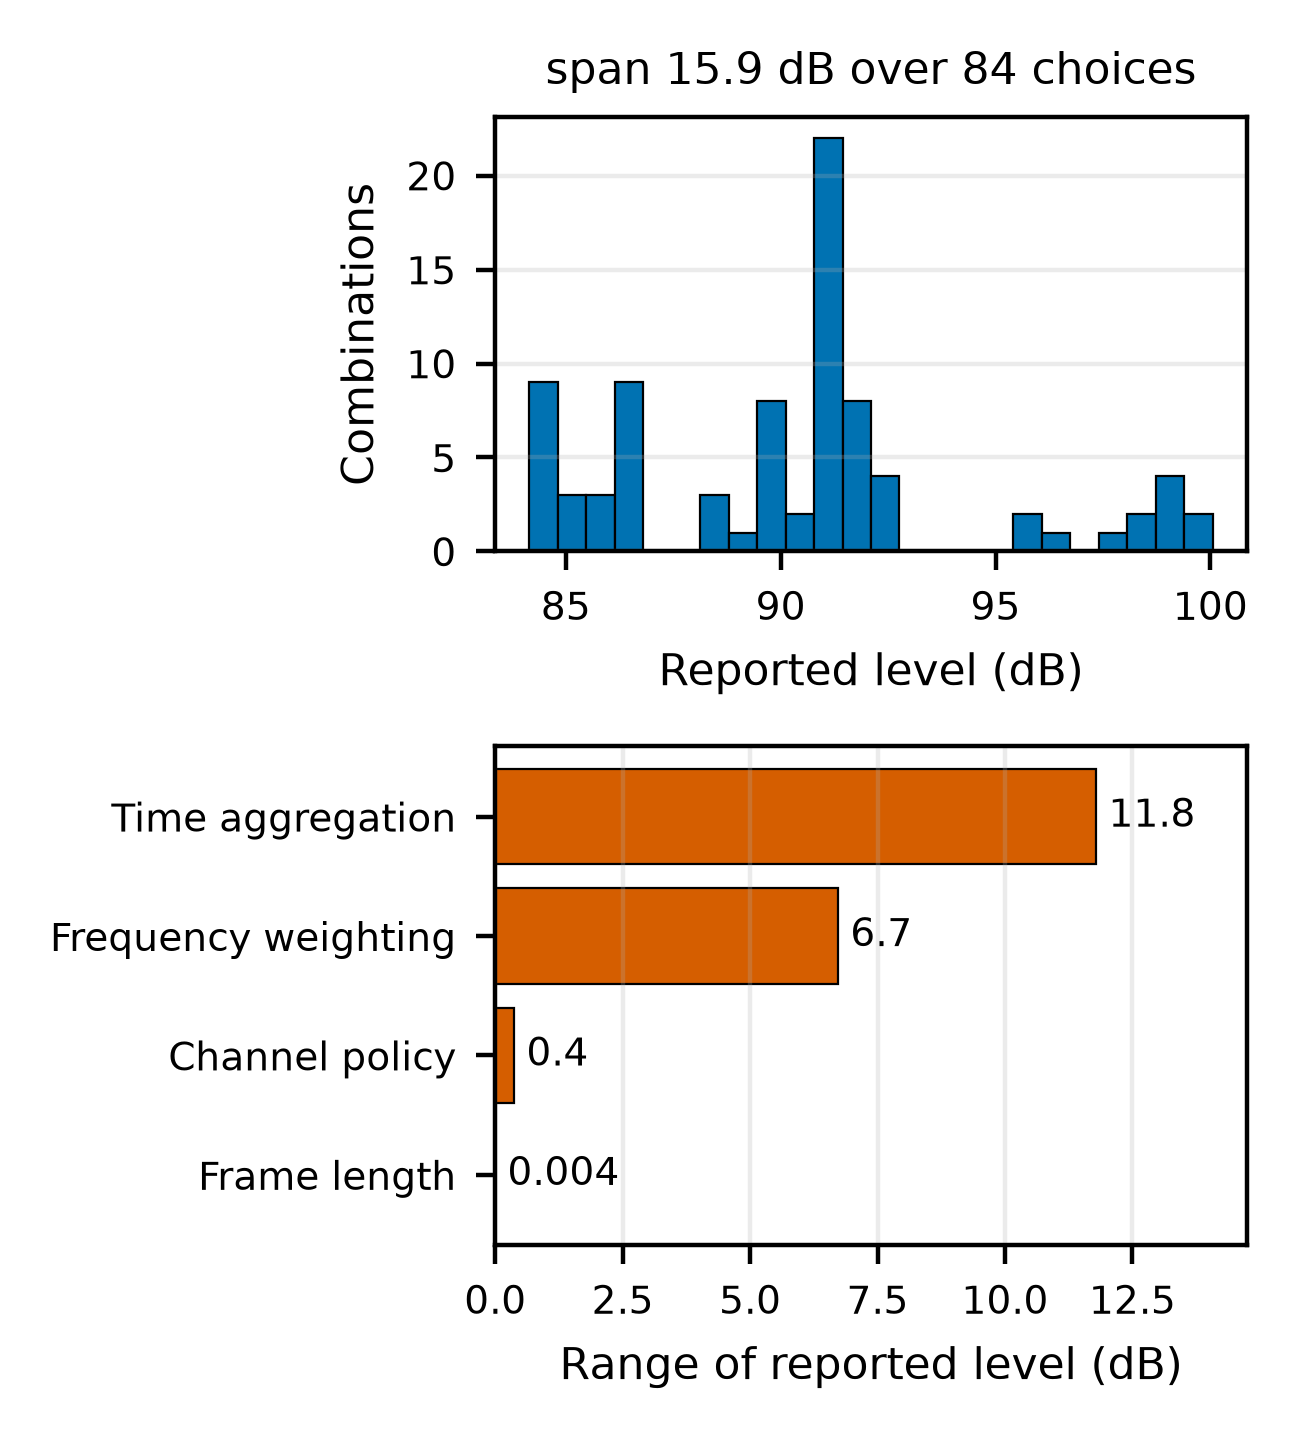
\includegraphics[width=\columnwidth]{figures/fig_provenance_dispersion.png}
\caption{Reported level for one unchanged recording across \dispCombos{} undocumented analysis choices (top), and the range contributed by each axis in isolation (bottom).}
\label{fig:dispersion}
\end{figure}

\begin{table}[t]
\caption{DISPERSION OF THE REPORTED LEVEL BY CHOICE AXIS}
\label{tab:axes}
\centering
\footnotesize
\begin{tabular}{@{}lrr@{}}
\toprule
Axis varied (others at default) & Levels & Range (dB)\\
\midrule
\inputrows{results/table_axes.tex}
\midrule
All axes crossed & \dispCombos & \dispRange\\
Time statistic fixed at $L_{\mathrm{eq}}$ & \dispConservativeCombos & \dispConservativeRange\\
\bottomrule
\end{tabular}
\end{table}

\subsection{Analytic Accuracy at the Default Configuration}

Across \anaCases{} sinusoid cases analyzed at the pipeline default framing, the maximum absolute RMS error was \anaRmsErr~dB, peak error \anaPeakErr~dB, and crest-factor error \anaCrestErr~dB. These are two orders of magnitude larger than the figures the previous revision reported, for the reason given below.

Spectral centroid behaves differently and the difference is the point. For tones centred on an analysis bin the worst centroid error was \anaCentroidOn~Hz; for tones offset by half a bin it was \anaCentroidOff~Hz, roughly \anaCentroidRatio{} times larger. Figure~\ref{fig:centroid} sweeps frame length and shows the two regimes separating as resolution changes. A previous revision of this evaluation reported a centroid error of 0.023~Hz, but obtained it with a frame length chosen so that every test tone completed an integer number of periods per frame --- a configuration no user running the defaults will encounter. The accuracy of a leakage-sensitive descriptor is a property of the analysis parameters, not of the implementation, and should be quoted with them.

\begin{figure}[t]
\centering
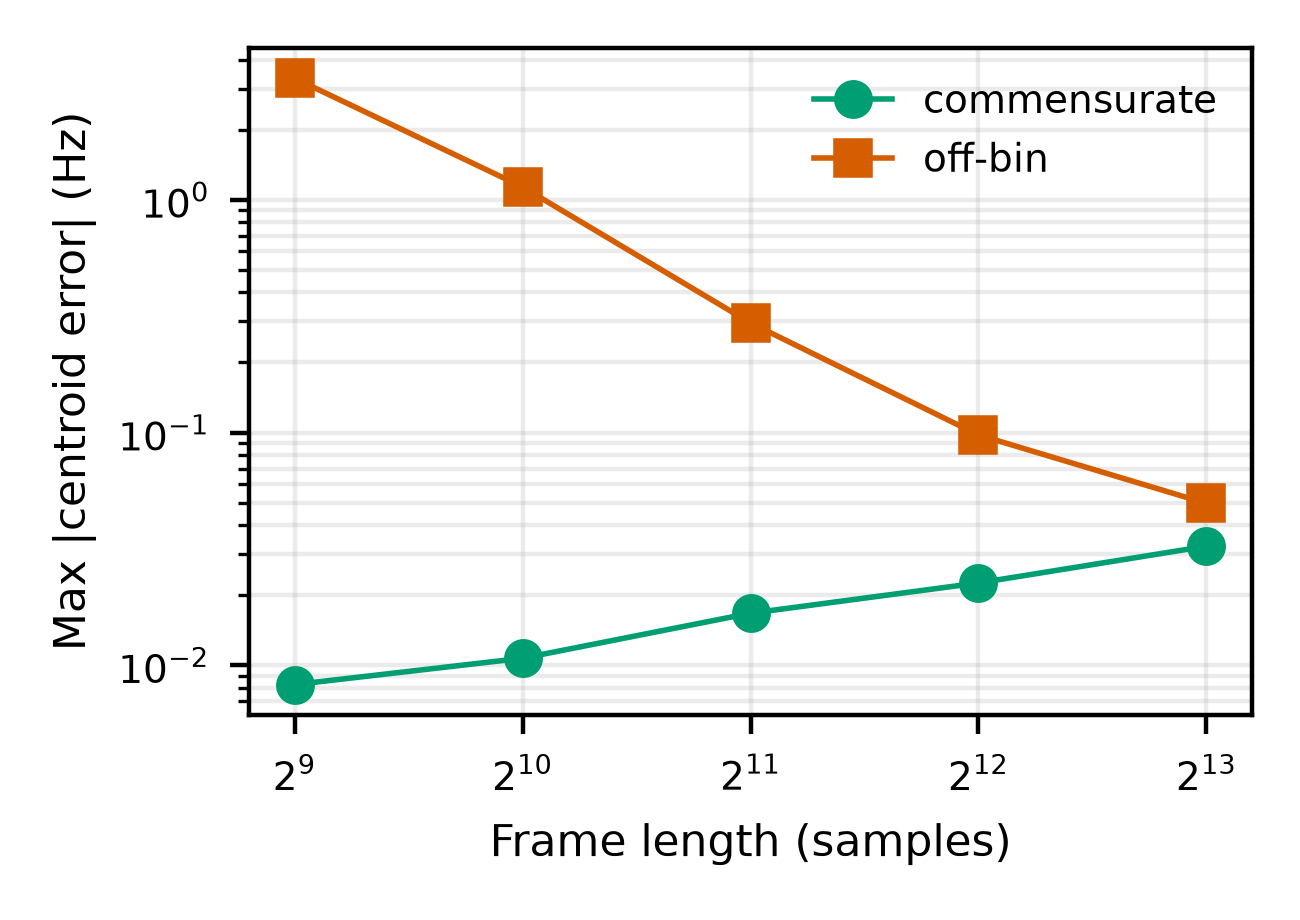
\includegraphics[width=\columnwidth]{figures/fig_centroid_framing.png}
\caption{Worst-case spectral centroid error against frame length, for tones on a bin centre and tones offset by half a bin.}
\label{fig:centroid}
\end{figure}

\subsection{Decay Estimation and Where It Fails}

For noiseless single-slope decays the maximum absolute $T_{30}$ error was \decayCleanErr~s, confirming the arithmetic of the Schroeder integration and the ISO 3382-1 $-5$ to $-35$~dB evaluation window \cite{schroeder1965,iso3382}. That result establishes almost nothing about in-situ measurement, because the implementation performs no Lundeby-style truncation of the integration at the noise floor \cite{lundeby1995}.

Adding a noise floor shows the consequence. Across the noisy single-slope cases the worst $T_{30}$ error was \decayWorstPct\%. Of the \decayDegraded{} cases in which the error exceeded 5\%, the decay validity test described in Sec.~\ref{sec:validity} marked \decayDegradedFlagged{} unavailable, on the grounds of insufficient dynamic range or an unsupported fit. The estimator is therefore not silently wrong on these inputs, but it is also not usable on them, and a user needing reverberation times from noisy in-situ impulse responses should treat noise-floor truncation as a prerequisite rather than an enhancement.

\subsection{Spatial Fixtures}
\label{sec:spatial}

Table~\ref{tab:spatial} summarizes the spatial results. The delayed-channel case is the one that matters. A 12-sample delay of the second channel yields a zero-lag correlation of $-0.0004$ --- indistinguishable from uncorrelated --- while the magnitude-squared coherence is 0.9995 and the lag-searching cross-correlation coefficient is 0.9939. The channels are almost perfectly coherent; they simply are not aligned. The earlier implementation, which reported the zero-lag correlation under the name coherence, made that statement impossible: its ``coherence'' of $-0.0004$ invited the reader to conclude the opposite of the truth.

Independent noise gives near-zero coherence and a low correlation coefficient, and its delay estimate of $34.3~\mu$s is now marked unavailable by the peak-to-sidelobe test of Eq.~\eqref{eq:psr} rather than left for the reader to disregard. The partially correlated pair sits where it should, between the two.

\begin{table*}[t]
\caption{SPATIAL FIXTURE RESULTS. THE DELAY IS THE SHIFT APPLIED TO CHANNEL 2 TO ALIGN IT WITH CHANNEL 1.}
\label{tab:spatial}
\centering
\small
\begin{tabular}{@{}lrrrrrrc@{}}
\toprule
Case & Target $\hat{\tau}$ ($\mu$s) & Measured $\hat{\tau}$ ($\mu$s) & ILD (dB) & Zero-lag corr. & MSC $\Gamma^2$ & IACC & $\hat{\tau}$ valid\\
\midrule
\inputrows{results/table_spatial.tex}
\bottomrule
\end{tabular}
\end{table*}

\subsection{Does the Validity Contract Fire?}
\label{sec:validity}

A contract that promises to distinguish an unavailable measurement from a real one is only worth what it can be shown to do. Six degenerate inputs were presented to six metrics, with the expected outcome for each of the \valCases{} pairs declared before the run. Of the \valExpected{} pairs where a metric genuinely had nothing to report, \valCorrect{} were marked unavailable. There were \valFalseAlarms{} false alarms: no metric declined to report a value it was entitled to report. Table~\ref{tab:validity} gives the matrix.

Reaching that result required changes prompted by the experiment itself, and they are worth stating rather than absorbing silently. In the first run, the spectral centroid returned approximately 12~kHz for digital silence, the arg-max of a spectrum consisting entirely of the additive floor $\epsilon_{\mathrm{mag}}$; the decay metrics returned a confident 2.9~s reverberation time for a DC offset; and the delay estimator reported an infinite peak-to-sidelobe ratio for an all-zero correlation surface. Each of these is a value that looks like a measurement, and none was. A silence test on Eq.~\eqref{eq:centroid}, the decay dynamic-range and slope test of Sec.~5.3, and a zero-peak guard on Eq.~\eqref{eq:psr} were added in response.

\begin{table}[t]
\caption{VALIDITY OUTCOMES ON DEGENERATE INPUTS}
\label{tab:validity}
\centering
\footnotesize
\begin{tabular}{@{}lrr@{}}
\toprule
& Reported a value & Marked unavailable\\
\midrule
Should be unavailable & \valMissed & \valCorrect\\
Should report a value & \valCorrectReported & \valFalseAlarms\\
\bottomrule
\end{tabular}
\end{table}

\subsection{Event Localization}

With boundaries drawn uniformly rather than placed on the hop grid, tone-to-tone transitions in the absence of noise were localized with a median absolute error of \evtCleanMedian~ms against a hop of \evtHopMs~ms, and \evtCleanRate\% of trials landed within one frame of the true boundary (Fig.~\ref{fig:event}). Errors of roughly half a hop are what uniform boundary placement predicts and are a property of the analysis grid, not of the detector.

The informative result is what happens in noise, and the median hides it. At 0~dB signal-to-noise ratio the tone-to-tone median stays at \evtNoisyMedian~ms while the 95th percentile rises to \evtNoisyPninetyfive~s: most trials still localize well and roughly a fifth fail outright, so the within-one-frame rate falls to \evtNoisyRate\%. Level steps degrade furthest, from \evtCleanMedianStep~ms with no noise to a \evtNoiseRateStep\% detection rate and a median error of \evtNoiseMedianStep~s at 0~dB, which is the expected weakness of a spectral-flux detector: a change in level with no change in spectral shape is close to invisible to it. Detection rate and an upper percentile, not a median, are the statistics to quote for this measure.

The previous revision of this evaluation reported a localization error of exactly 0~ms. It placed its transitions at 4.000 and 8.000~s, which at a 16~kHz sample rate and a 256-sample hop are hop indices 250 and 500 exactly; zero error was arithmetically unavoidable and the experiment could not have produced any other number.

\begin{figure}[t]
\centering
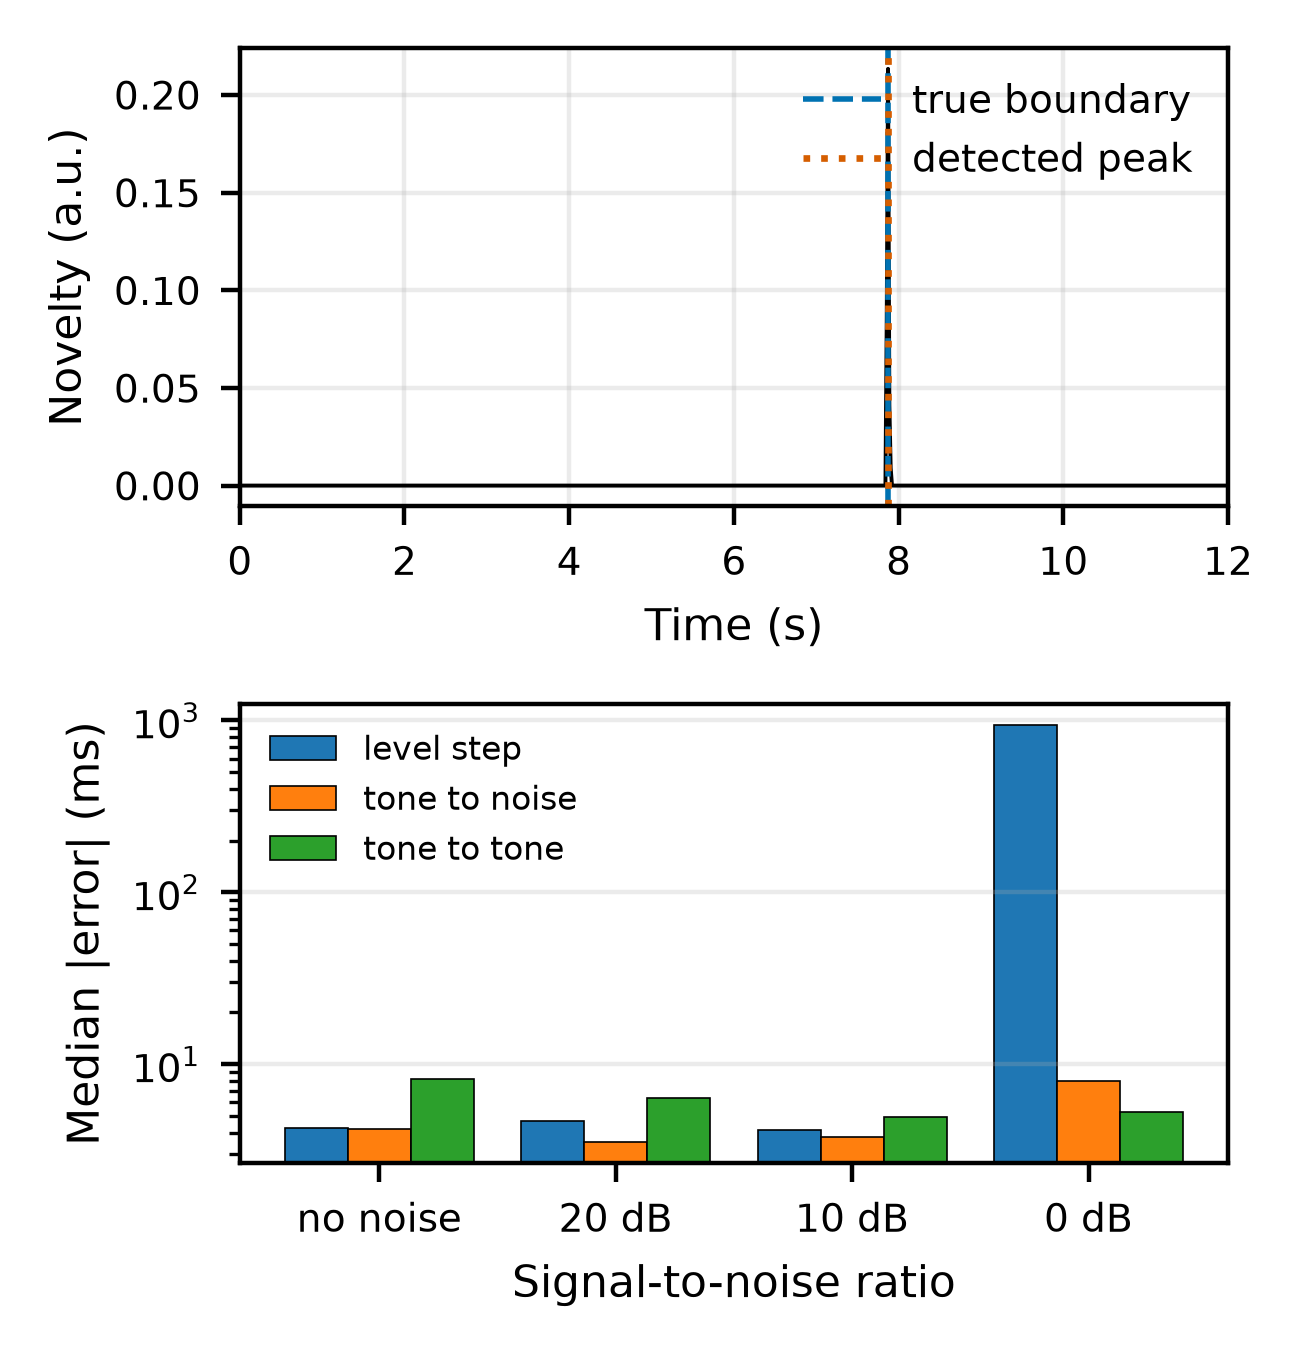
\includegraphics[width=\columnwidth]{figures/fig_event_localization.png}
\caption{Novelty response for one trial (top) and median absolute localization error by transition type and signal-to-noise ratio over \evtTrials{} trials per condition (bottom).}
\label{fig:event}
\end{figure}

\subsection{Streaming: Frame Accounting and Agreement}
\label{sec:streaming}

Independent chunking discarded between \streamLegacyMissingMin\% and \streamLegacyMissing\% of frames depending on chunk size and metric, and the surviving frames were not a subset of the full-file frames but a re-anchored grid. The resulting summary-mean discrepancy reached \streamLegacyWorstRel\% on the novelty curve.

With the frame-aligned path of Sec.~\ref{sec:streaming-design}, all \streamChecked{} metric-by-chunk-size comparisons produced series bit-identical to full-file analysis: no frames missing, and a maximum absolute per-frame difference of exactly zero. Table~\ref{tab:agreement} contrasts the two strategies. This is a stronger statement than the mean agreement reported previously, and it is stronger in the way that matters: equal means do not imply equal series, and a summary statistic can hide a systematically displaced frame grid.

The result should not be over-read. It holds for the \eslMetricStreaming{} metrics that declare chunk compatibility, at chunk sizes of at least one frame. Metrics requiring global normalization, long integration histories, or whole-signal impulse-response structure remain excluded from the streaming path by the scheduler rather than approximated within it.

\begin{table}[t]
\caption{STREAMING AGREEMENT WITH FULL-FILE ANALYSIS}
\label{tab:agreement}
\centering
\footnotesize
\begin{tabular}{@{}lrr@{}}
\toprule
& Independent & Frame-\\
& chunks & aligned\\
\midrule
Frames missing (max) & \streamLegacyMissing\% & 0\%\\
Series identical to full file & no & \streamIdentical\\
Max per-frame difference & --- & 0\\
Worst mean difference & \streamLegacyWorstRel\% & 0\%\\
\bottomrule
\end{tabular}
\end{table}

\subsection{Memory Scaling and Its Causes}
\label{sec:memory}

Peak resident memory is not linear in duration from zero. Every run in this sweep, in both modes, sits on a floor of \memFloor~MiB set by the interpreter and its imported libraries, and below \memFloorBelow~s of audio that floor is all one measures. Above it, full-file memory is linear with a slope of \memFullSlope~MiB per second of stereo 48~kHz audio over the \memFitPoints{} points that have left the floor ($r^2=\memFullRsq$). The streaming path never leaves the floor: it holds \memStreamIntercept~MiB from 15~s to \memMaxDuration~s of input, with no measurable growth (Fig.~\ref{fig:memory}).

Reporting this as a percentage, as the previous revision of this work did, is a mistake twice over. A percentage reduction is a property of the duration chosen for the benchmark rather than of the architecture, tending to zero for short files and to 100\% for long ones; and at the durations where the floor dominates, it measures the size of the Python interpreter rather than anything about the analysis. The slope is the architectural quantity. It implies roughly \memFullHour~GiB of resident memory to analyze one hour of stereo audio in full-file mode and about \memFullDay~GiB for a day, against a constant \memStreamIntercept~MiB for the streaming path. Those two figures are extrapolations from a fitted line, not measurements, and Sec.~\ref{sec:limits} says so again.

The slope is \memDataRateMultiple{} times the raw stereo float32 data rate of 0.366~MiB/s, which invites the question of where it goes. Table~\ref{tab:budget} accounts for it from the arrays the pipeline holds. If every array were resident simultaneously the cost would be \memPredicted~MiB/s, an upper bound the measurement does not reach; the complex transform, its magnitude, and the decoded waveform alone come to \memPredictedSubset~MiB/s, which brackets the measured \memFullSlope~MiB/s from below. The framed time-domain buffer is therefore evidently not live at the same instant as the spectral arrays. What is unambiguous is that the retained metric series --- the component a reader might reasonably assume streaming exists to eliminate --- account for under 0.2\% of the growth. The practical implication is that streaming is not the only remedy available: single-precision spectral storage would remove about half the slope, and that is a cheaper change than restructuring an analysis to be chunk-compatible.

\begin{table}[t]
\caption{FULL-FILE MEMORY BUDGET PER SECOND OF STEREO AUDIO}
\label{tab:budget}
\centering
\footnotesize
\begin{tabular}{@{}lr@{}}
\toprule
Component & MiB/s\\
\midrule
\inputrows{results/table_budget_components.tex}
\midrule
\inputrows{results/table_budget_totals.tex}
\bottomrule
\end{tabular}
\end{table}

\begin{figure}[t]
\centering
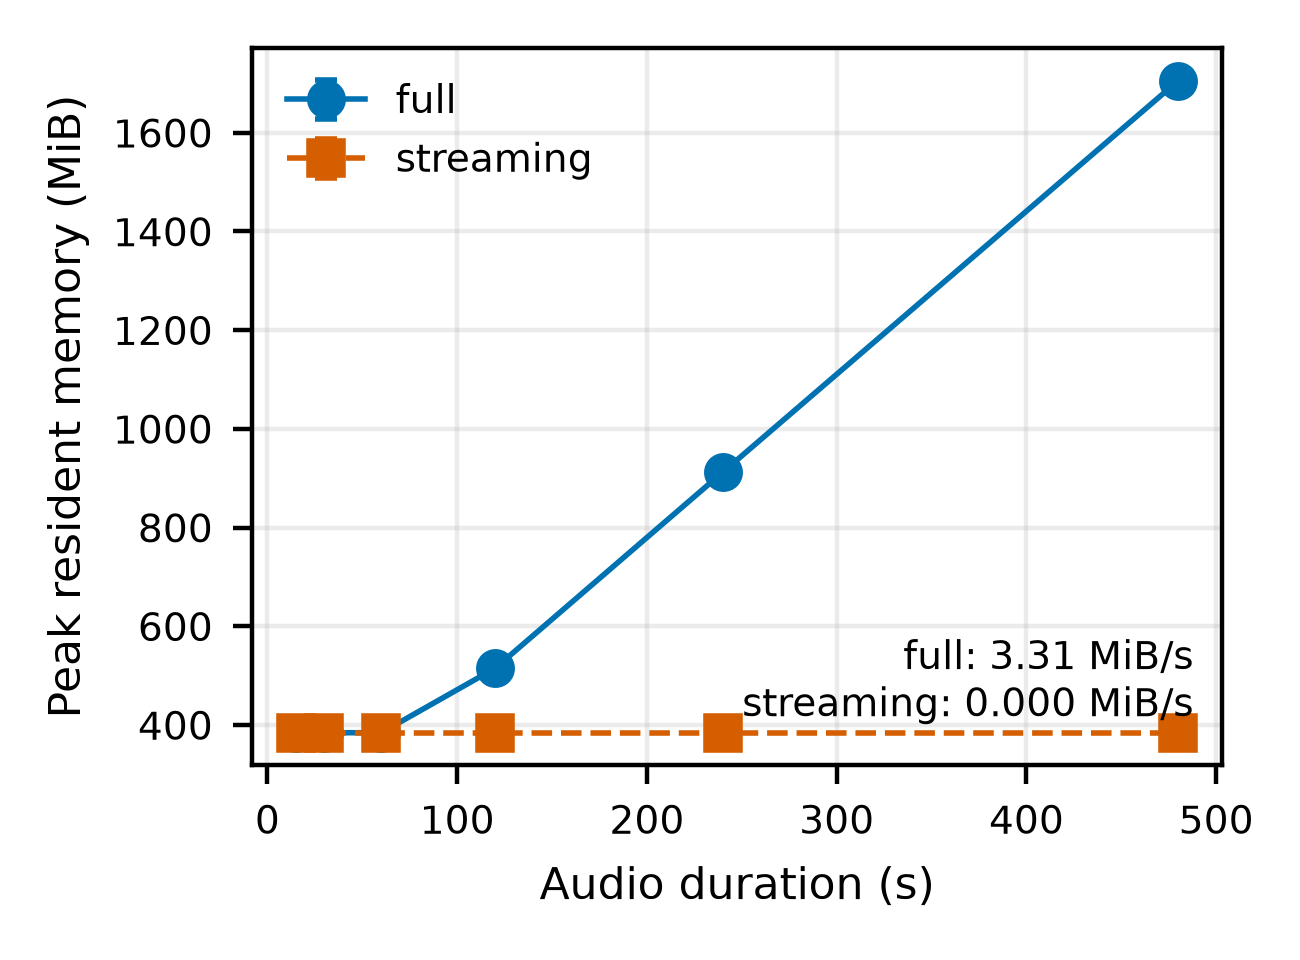
\includegraphics[width=\columnwidth]{figures/fig_memory_scaling.png}
\caption{Peak resident memory against audio duration, three runs per point, measured in separate processes. Error bars show the range across repeats.}
\label{fig:memory}
\end{figure}

\subsection{Calibration}

All \calFixtures{} calibration fixtures passed at the tightened tolerance of \calTolerance~dB, with a maximum observed level error of \calAchieved~dB. These fixtures validate the software mapping from digital level to physical level, not the traceability or uncertainty of any physical measurement chain.

\section{DISCUSSION}

\subsection{What the Evaluation Establishes}

The dispersion result of Sec.~\ref{sec:dispersion} is the substantive finding. It converts the paper's motivating claim from an assertion into a measurement: on one ordinary nonstationary signal, the choices that a bare reported level omits are worth \dispConservativeRange~dB even when the time statistic is held fixed. Any workflow that reports levels without those choices is transmitting a number with that much slack in it, and no amount of arithmetic precision in the estimator recovers it.

The remaining results test the four contributions rather than restating them. Streaming is now numerically identical to full-file analysis for its declared metrics, so a user is not asked to trade correctness for memory. The validity fields fire on \valCorrect{} of \valExpected{} degenerate cases with no false alarms --- but reaching that number required fixing three metrics that returned confident nonsense, which is the strongest available argument for running the experiment rather than describing the design.

The naming audit deserves particular emphasis because it cuts against the paper's own earlier draft. A workflow whose stated purpose is to keep names, units and conditions attached to values had itself published a correlation coefficient under the name coherence for several releases, and the error was visible in a results table as a negative value of a non-negative quantity. Two conclusions follow. The first is narrow: the metric is fixed, the old name survives as a warning-emitting alias, and a real magnitude-squared coherence now exists alongside it. The second is general: a result contract is not self-enforcing. It needs fixtures that would expose a violation, and the ones that found this were fixtures designed so that theory predicts a specific disagreement between two statistics.

\subsection{Limitations}
\label{sec:limits}

Six limitations constrain the conclusions. First, all reported fixtures are synthetic. They do not span field noise, recorder clock drift, codec artifacts, weather protection, microphone self-noise, or uncertain geometry. Second, no result here is validated against an independent implementation. Agreement with a reference implementation --- the EBU Tech 3341 compliance signals for loudness \cite{ebu3341}, the IEC 61672 tolerance envelopes for weighting \cite{iec61672}, established index implementations for the ecoacoustic group \cite{ulloa2021,sueur2008} --- would test claims that self-consistency cannot, and its absence is the largest single gap in this paper. Third, the calibration checks validate software mappings, not the traceability or uncertainty of a physical measurement chain, and no uncertainty budget is offered. Fourth, the room-acoustic tests use synthetic decays; measured impulse responses with real noise floors, multiple slopes, and octave-band filtering per IEC 61260 remain untested \cite{iec61260}. Fifth, spatial verification is limited to two-channel pairs; despite the presence of ambisonic metrics in the registry, no higher-order or object-based material was evaluated, and the paper's claims should be read as applying to mono and stereo signals only. Sixth, the memory benchmark reaches \memMaxDuration~s on one host; the one-hour and one-day figures are extrapolations from a fitted line, not measurements, and operating-system accounting differs across platforms.

Further work should add openly licensed field corpora with independent annotations, cross-implementation agreement tables, measurement uncertainty budgets, codec and sample-rate stress tests, and multichannel reference scenes. Noise-floor truncation for decay estimation and single-precision spectral storage are both small changes with measurable consequences identified above.

\subsection{Reproducibility and Availability}

The source package, evaluation script, generated CSV and JSON files, figures, and manuscript source are distributed in the ecoSignalLab repository at \url{https://github.com/TheColby/ecoSignalLab}. The evaluated revision is \texttt{\eslCommitFull}. Running \texttt{uv run python paper/evaluation.py} from the repository root regenerates every evidence artifact, including \texttt{results/numbers.tex}, from which this manuscript takes every quantity it quotes; a number in this paper therefore cannot disagree with the run that produced it. Running the repository test suite at the same revision completed successfully; these tests are software regression evidence and are not a replacement for the external validations proposed above.

The software is distributed under the MIT License. Since operating-system memory accounting and library versions affect the absolute benchmark values, reproduction should compare scaling trends and numeric agreement in addition to raw MiB and timing values.

\section{CONCLUSION}

A sound level reported without its analysis context carries a spread of \dispConservativeRange~dB on the signal measured here, and \dispRange~dB once the choice of time statistic is admitted. ecoSignalLab binds each of \eslMetricTotal{} metrics to the framing, channel, calibration, and validity context that produced it, and this paper tests that binding rather than describing it. A frame-aligned streaming path is bit-identical to full-file analysis across all \streamChecked{} comparisons made, removing the correctness penalty that chunked execution previously carried, while peak memory stays at \memStreamIntercept~MiB against a full-file growth of \memFullSlope~MiB per second of stereo audio. Validity fields correctly declined to report \valCorrect{} of \valExpected{} degenerate cases with no false alarms. An audit against the project's own contract found and corrected a metric published for several releases under a name it did not deserve, which is the clearest evidence in this paper both for the value of the contract and for the necessity of testing it. What remains is external validation: agreement with independent implementations, field material, and an uncertainty budget. The supplied artifacts are intended to make that work straightforward to attach.

\section*{ACKNOWLEDGMENT}

Anthropic Claude (Opus 5) was used in preparing this revision: it reviewed the previous draft, proposed and implemented the software changes described in Secs.~\ref{sec:streaming-design} and \ref{sec:spatial-design}, redesigned the evaluation script, and drafted manuscript text. OpenAI Codex (GPT-5) assisted with the initial draft, evaluation-code scaffolding, and figure layout. The author directed the work, reviewed and verified all text, data, figures, references, and interpretations, and is solely responsible for the content. No external funding supported this work.

\bibliographystyle{jaes}
\bibliography{references}

\biography{Colby Leider}{figures/esl_author_mark.png}{Colby Leider is the lead developer of the ecoSignalLab open-source project. His audio-engineering work includes environmental acoustic monitoring, multisensor field systems, and reproducible signal-analysis workflows. He coauthored an AES Convention paper on wireless multisensor monitoring of the Florida Everglades.}

\end{document}
